\documentclass[10pt]{beamer}



\usepackage{amsmath, amssymb}
\usepackage{algorithm,algorithmic} 
\usepackage{tikz}
\newtheorem{assumption}{Assumption}
\setbeamertemplate{theorems}[numbered]
\setbeamertemplate{lemma}[numbered]
\setbeamertemplate{caption}[numbered]
\usepackage{multirow}
\usepackage{array}
\usefonttheme{professionalfonts}
\setbeamertemplate{navigation symbols}{}
\newcommand{\cref}[1]{{\color{blue}\footnotesize [#1]}}
\usepackage{graphicx,subfigure}
\usepackage{tensor,stmaryrd,bm,cases}
\usepackage{soul}
\usepackage{booktabs}
\usepackage[most]{tcolorbox}

% --- Rounded blocks matching the reference slide style ---
\definecolor{llxBlockBlue}{RGB}{57,57,180}
\definecolor{llxBlockTitleBg}{RGB}{214,214,242}
\definecolor{llxBlockBodyBg}{RGB}{239,239,250}
\setbeamertemplate{blocks}[rounded][shadow=true]
\setbeamercolor{block title}{fg=llxBlockBlue,bg=llxBlockTitleBg}
\setbeamercolor{block body}{fg=black,bg=llxBlockBodyBg}
\setbeamerfont{block title}{size=\large,series=\mdseries}

\newcommand{\rrr}{\textcolor{red}}
\newcommand{\IiH}{\bm{\mathcal{H}}}
\newcommand{\IiM}{\bm{\mathcal{M}}}
\newcommand{\IiS}{\bm{\mathcal{S}}}
\newcommand{\bM}{\bm{M}}
\newcommand{\bx}{\mathbf{x}}

% Toggle backup slides without removing their source.
\newif\ifshowappendix
\showappendixfalse

% --- page number ---
\setbeamertemplate{footline}{%
	\raisebox{10pt}{\makebox[\paperwidth]{\hfill\makebox[7em]{\normalsize\texttt{\insertframenumber/\inserttotalframenumber}}}}%
}

% Insert an unnumbered section title page before every section.
\AtBeginSection[]{%
    \begin{frame}[plain,noframenumbering]
        \vfill
        \begin{beamercolorbox}[sep=12pt,center]{section title}
            \usebeamerfont{section title}\secname
        \end{beamercolorbox}
        \vfill
    \end{frame}%
}


\begin{document}  

\newtheorem{thm}{Theorem}[section]   %thm:定理
\newtheorem{cor}{Proposition} %cor:假设
\newtheorem{pro}{Problem}   %pro：问题
\newtheorem{dfn}{Definition}  %dfn:定义
\newtheorem{rmk}{Remark}  %rmk:标记
\newtheorem{prf}{Proof}   %prf:证明
\newtheorem{lem}{Lemma}[section]

\newcommand{\red}[1]{{\color[rgb]{1,0,0}{#1}}}
\newcommand{\blue}[1]{{\color[rgb]{0,0,1}{#1}}}
\newcommand{\green}[1]{{\color[rgb]{0,1,0}{#1}}}
\newcommand{\cg}[1]{{\colorbox{green}{#1}}}
\newcommand{\cy}[1]{{\colorbox{yellow}{#1}}}


\title{Deterministic Oracle Complexity of Nonsmooth Difference-of-Convex Optimization} 
\author{Discussion with Prof.\ Anthony Man-Cho So \\[4pt] Presenter: Luxuan Li}
% \author{}
\date{Aug 21, 2026}
\maketitle

\begin{frame}{Outline}

\begin{enumerate}\setlength{\itemsep}{6pt}
    \item[\textbf{I.}] \textbf{Research Goal}\\[-1pt]


    \item[\textbf{II.}] \textbf{Preliminaries}\\[-1pt]


    \item[\textbf{III.}] \textbf{Discussion}\\[-1pt]
  

    \item[\textbf{IV.}] \textbf{Future Work}\\[-1pt]

\end{enumerate}
\end{frame}

\section{I. Research Goal}

\begin{frame}{Nonsmooth DC Optimization Problem}
\small
\[
    F(x)=\phi(x)-g(x),
    \qquad
    \phi,g\in\Gamma_0(\mathbb R^d).
\]
Here $\Gamma_0(\mathbb R^d)$ denotes proper, closed, convex functions.

\begin{itemize}\setlength{\itemsep}{2pt}
    \item $F$ is $L$-Lipschitz on $\mathbb R^d$
    % \item $F+\frac{\rho}{2}\|\cdot\|^2$ is convex when weak convexity is used;
    \item the initialization gap is
    $\Delta_0=F(x^0)-\inf_xF(x)<\infty$.
    \item g is nonsmooth 
\end{itemize}

% \begin{alertblock}{Focus}
%     A unified oracle complexity analysis for nonsmooth DC optimization.
% \end{alertblock}

\vspace{0.08cm}
\begin{alertblock}{Research Question}
How can we
design a complexity-analysis framework for nonsmooth DC optimization based on
a unified and computable oracle model?
\end{alertblock}
\end{frame}

% \section{Background}

% % \begin{frame}{Stationarity in Nonsmooth (DC) Optimization}
% % \footnotesize
% % \vspace{0.2cm}
% % \begin{itemize}\setlength{\itemsep}{2pt}
% %     \item \textbf{Clarke stationarity} (conventional target): one seeks
% %     $$
% %     0\in\partial_C F(\bar x).
% %     $$
% %     \item \textbf{Critical point in DC optimization:}
% %     $\bar x$ is a critical point of Problem (P) if
% %     $$
% %     0\in\partial\varphi(\bar x)-\partial g(\bar x),
% %     \quad\text{equivalently,}\quad
% %     \partial\varphi(\bar x)\cap\partial g(\bar x)\neq\emptyset.
% %     $$
% %     \item \textbf{Relation:}
% %     $$
% %     \partial_C(\varphi-g)(x)\subseteq\partial\varphi(x)-\partial g(x).
% %     $$
% % \end{itemize}
% % \end{frame}

    
% % \begin{frame}{Asymptotic Stationarity vs.\ Finite-Time Convergence}
% % \small
% % For locally Lipschitz $F$, a typical asymptotic convergence proof gives
% % \[
% %     x^k\to x^\star,
% %     \qquad
% %     0\in\partial_C F(x^\star),
% % \]
% % but \emph{not} $\operatorname{dist}(0,\partial_C F(x^k))\to0$, and no finite
% % $K(\varepsilon)$ with $\operatorname{dist}(0,\partial_C F(x^K))\le\varepsilon$
% % is guaranteed to exist.

% % \begin{alertblock}{Key reason}
% % At a nonsmooth point, the subdifferential set may expand abruptly:
% % $F(x)=|x|$ has $0\in\partial_C F(0)=[-1,1]$, yet
% % $\operatorname{dist}\bigl(0,\partial_C F(x)\bigr)=1$ for all $x\neq0$.
% % \end{alertblock}

% % \medskip
% % \textbf{Finite-time Convergence Criteria in DC optimization.}
% % \begin{itemize}\setlength{\itemsep}{1pt}
% %     \item \textbf{Critical point:}
% %     $0\in\partial\varphi(\bar x)-\partial g(\bar x)$;
% %     \item \textbf{Finite-time relaxation:} Given $\varepsilon>0$,
% %     $\varepsilon$-criticality means
% %     $$
% %     \operatorname{dist}\!\left(0,\partial\varphi(\bar x)-\partial g(\bar x)\right)\le\varepsilon.
% %     $$
% % \end{itemize}

% % \medskip
% % \red{\textbf{Question 1.}}\quad
% % Can any finite-time algorithm return an \red{\emph{exact}} same-point $\varepsilon$-critical point of Problem (P)?
% % \end{frame}
% % \begin{frame}{Asymptotic Stationarity vs.\ Finite-Time Convergence}
% % \small
% % For a locally Lipschitz nonsmooth objective \(F\), consider an algorithm
% % \(\mathcal A\) generating \(\{x^k\}_{k\in\mathbb N}\).

% % \medskip
% % \textbf{1. Asymptotic guarantee.}

% % A typical convergence result proves
% % \[
% %     x^k \to x^\star,
% %     \qquad
% %     0\in \partial_C F(x^\star).
% % \]

% % \medskip
% % \textbf{2. Finite-time target.}

% % Given \(\varepsilon>0\), can we find a finite
% % \(K=K(\varepsilon)\) such that
% % \[
% %     \operatorname{dist}
% %     \bigl(0,\partial_C F(x^K)\bigr)
% %     \le \varepsilon?
% % \]

% % \medskip
% % The asymptotic statement does not imply
% % \[
% %     \operatorname{dist}
% %     \bigl(0,\partial_C F(x^k)\bigr)\to 0
% %     \qquad \text{as } k\to\infty,
% % \]
% % nor does it guarantee that there exists an index
% % \(k^0\in\{1,\ldots,K\}\) such that
% % \[
% %     \operatorname{dist}
% %     \bigl(0,\partial_C F(x^{k^0})\bigr)\le \varepsilon.
% % \]

% % \begin{alertblock}{Key reason}
% % At a nonsmooth point, the subdifferential set may expand abruptly.

% % For example, $F(x) = |x|$, $0 \in \partial_C F(0) = [-1,1]$ but $\operatorname{dist}\bigl(0,\partial_C F(x)\bigr)=1,\quad x>0$.
% % \end{alertblock}

% % \end{frame}

% % [2026-07-29] The standalone asymptotic-vs-finite-time frame was merged into
% % the preceding frame (general part + DC finite-time criteria + Question 1).


% % \begin{frame}{The Same Obstruction in Nonsmooth DC Optimization}
% % \vspace{0.2cm}

% % \begin{columns}[T,onlytextwidth]

% % \column{0.58\textwidth}

% % Consider the DC example
% % \[
% %     \Psi(x)=\bigl||x|-1\bigr|
% %     =\phi(x)-g(x),
% % \]
% % with
% % \[
% %     \phi(x)=3+4(|x|-1)_+,
% % \]
% % \[
% %     g(x)=|x+1|+|x|+|x-1|.
% % \]

% % \column{0.38\textwidth}

% % \centering
% % \vspace{-0.8em}

% % \begin{tikzpicture}[x=0.75cm,y=1.25cm,>=stealth]

% %     \draw[->] (-2.25,0) -- (2.25,0) node[right] {$x$};
% %     \draw[->] (0,-0.15) -- (0,1.35) node[above] {$\Psi(x)$};

% %     \draw[very thick,blue!70!black]
% %         (-2,1) -- (-1,0) -- (0,1) -- (1,0) -- (2,1);

% %     \fill[red!70!black] (-1,0) circle (2pt);
% %     \fill[red!70!black] (1,0) circle (2pt);

% %     \node[below] at (-1,0) {$-1$};
% %     \node[below] at (1,0) {$1$};
% %     \node[left] at (0,1) {$1$};

% % \end{tikzpicture}

% % \end{columns}

% % \vspace{0.2cm}
% % \medskip
% % \begin{itemize}
% % \item For \(x_k=1-\frac{1}{k+2}\),
% % \[
% %     x_k\to1,
% %     \qquad
% %     0\in\partial\phi(1)-\partial g(1),
% % \]
% % while every finite iterate satisfies
% % \[
% %     \operatorname{dist}
% %     \bigl(0,\partial\phi(x_k)-\partial g(x_k)\bigr)=1.
% % \]
% % \end{itemize}
% % \begin{alertblock}{Consequence}
% % Convergence to a DC-critical point does not ensure that the exact
% % same-point residual becomes small along the finite trajectory.
% % \end{alertblock}
% % % \medskip
% % % \centering
% % % \textbf{This motivates a finite-time reachable relaxed DC stationarity.}

% % \end{frame}

% \begin{frame}{Unattainability of the $\varepsilon$-Critical Point}
% For general nonsmooth nonconvex optimization,
% Zhang et al.\footnote{
% J.~Zhang, H.~Lin, S.~Jegelka, S.~Sra, and A.~Jadbabaie,
% \emph{Complexity of Finding Stationary Points of Nonsmooth
% Nonconvex Functions}, ICML, 2020, Theorem~5.
% } showed that $\varepsilon$-Clarke stationarity is not finitely attainable.

% \vspace{0.2cm}
% \medskip
% In nonsmooth DC optimization this obstruction is \emph{not} inherited
% automatically:
% \begin{itemize}\setlength{\itemsep}{1pt}
%     \item the DC oracle is \emph{stronger}: it may reveal
%           $\partial\phi(x)$ and $\partial g(x)$ separately;
%     \item the DC residual is \emph{weaker}:
%           $\partial_C(\phi-g)(x)\subseteq \partial\phi(x)-\partial g(x)$,
%           hence
%           $\operatorname{dist}(0,\partial\phi-\partial g)\le
%            \operatorname{dist}(0,\partial_C(\phi-g))$.
% \end{itemize}
% \end{frame}

% \section{Preliminaries}


% % \begin{frame}{Unattainability of the $\varepsilon$-Critical Point}
% % \small
% % To answer \red{Question 1}, we offer two approaches to hard instances built with GPT’s assistance.

% % \vspace{0.2cm}
% % \medskip
% % \textbf{Theorem A.} There is an \emph{absolute} constant $c_0>0$ such that, for every finite
% % $K$, every $\varepsilon\in\bigl(0,\,c_0\min\{L,G\}\bigr]$, and every
% % (possibly randomized) algorithm $\mathcal A$ interacting with
% % $\mathcal O_{\rm DC}$, there exists $(\phi,g)\in\mathcal D(\Delta,L,G)$
% % with \blue{$(\Delta,L,G)$ independent of $K$} such that, w.p.\ $\ge 1/2$,
% % $$
% %     \operatorname{dist}\!\bigl(0,\partial\phi(x^k)-\partial g(x^k)\bigr)
% %     >\varepsilon,\qquad k=1,\dots,K.
% % $$
% % Moreover, the critical point the pair contains $z^\star$ with
% % $0\in\partial\phi(z^\star)-\partial g(z^\star)$ but $0\notin\partial_C(\phi-g)(z^\star)$.

% % \end{frame}


% % 但这个反例感觉还没有被完全证明

% % \begin{frame}{Unattainability of the $\varepsilon$-Critical Point}
% % \small

% % \medskip
% % \textbf{Proof skeleton} (barrier by reduction from the convex small-subgradient LB\footnote{
% % G.~Kornowski and O.~Shamir,
% % \emph{On the Complexity of Finding Small Subgradients in
% % Nonsmooth Optimization},
% % NeurIPS 2022 Workshop; arXiv:2209.10346v2.
% % }):
% % \begin{enumerate}\setlength\itemsep{2pt}
% %   \item \textbf{Convex LB.} For 1-D convex $1$-Lipschitz $q$, no finite-time first-order algorithm guarantees $\operatorname{dist}(0,\partial q(x))\le\varepsilon$.
% %   \item \textbf{2-D lifting.}
% %   $$
% %      \phi_q(x,y)=q(x)+|y|+\blue{|y-1|},\quad g_q(x,y)=\blue{|y-1|},\quad F_q=\phi_q-g_q=q(x)+|y|.
% %   $$
% %   \item \textbf{Reduction validity.} $D(x,y):=\operatorname{dist}(0,\partial\phi_q-\partial g_q)\ge\operatorname{dist}(0,\partial q(x))$; 
% %   % component-wise DC oracle on the $x$-block $\equiv$ convex first-order oracle of $q$ ($y$-info fully known).
% %   \item \textbf{Strict separation.} At $(x^\star,1)$, $x^\star\in\arg\min q$: $0\in\partial\phi_q-\partial g_q$ but $\partial_C F_q(x^\star,1)=\partial q(x^\star)\times\{1\}\not\ni0$.
% %   \item \textbf{Parameters.} Fixed $(\Delta,L,G)=(1,\sqrt2,\sqrt5)$, $K$-independent; rescale by $\rho=\tfrac13\min\{L,G\}$ to arbitrary $(\Delta,L,G)$.
% % \end{enumerate}

% % \medskip
% % \red{\textbf{Limitation.}}
% % The hardness is inherited from a one-dimensional convex lower bound;
% % \end{frame}

% % \begin{frame}{Unattainability of the $\varepsilon$-Critical Point }
% % \footnotesize
% % \textbf{Theorem B.} Fix $\Delta,L,G>0$. There exists $c>0$ such that for \red{every $K\le cG/L$, every $\varepsilon\in(0,L)$}, and every $\mathcal A$ with oracle $\mathcal O_{\rm DC}$, there exists $(\phi,g)\in\mathcal D(\Delta,L,G)$ such that, w.p.\ $\ge1/2$,
% % $$
% %   \operatorname{dist}\bigl(0,\partial\phi(x^k)-\partial g(x^k)\bigr)>\varepsilon,\quad k=1,\dots,K.
% % $$
% % Moreover, the pair contains a point $s$ with $0\in\partial\phi(s)-\partial g(s)$ but $0\notin\partial_C(\phi-g)(s)$.


% % \vspace{0.2cm}
% % \medskip
% % \blue{\textbf{Answer 1.}}\quad
% % A traditional \red{exact} same-point $\epsilon$-critical point \red{cannot be
% % obtained} in finite time, even under the strong component-wise DC
% % oracle, returning values and subgradients of $\phi$ and $g$
% % separately.
% % \end{frame}

% % \begin{frame}
% % \footnotesize
% %   \textbf{Proof skeleton} (DC resisting oracle, adapted from Zhang et al. 2020):
% % \begin{enumerate}\setlength\itemsep{2pt}
% %   \item \textbf{Background.} $(\phi_0,g_0)$ with hidden kinks s.t.
% %   $$\operatorname{dist}\!\bigl(0,\partial\phi_0(x^k)-\partial g_0(x^k)\bigr)>\varepsilon,\quad \forall\,k.$$
% %   \item \textbf{Graft.} $c_s(x)=M|x-s|+\beta-Ms$;\ \ $\phi_s=\phi_0+c_s,\ g_s=g_0+c_s$. Two $s$-invariants:
% %   $$F_s:=\phi_s-g_s=\phi_0-g_0,\qquad c_s(x)=\beta-Mx\ \text{on }\{x<s\}.$$
% %   \item \textbf{Indistinguishability.} For every admissible $s>\max_k x^k$, the transcript $(\phi_s,g_s,\partial\phi_s,\partial g_s)\big|_{x^k}$ is $s$-invariant.
% %   \item \textbf{Separation.} At $x=s$, $\partial c_s(s)=[-M,M]$, hence
% %   $$0\in\partial\phi_s(s)-\partial g_s(s),\qquad 0\notin\partial_C F_s(s).$$
% % \end{enumerate}
% % Two admissible $s\neq s'$ share the same transcript $\Rightarrow$ $\Pr[\mathrm{fail}]\ge\tfrac12$.

% % \medskip
% % \alert{Limitation:} requires $K\le cG/L$ (equiv.\ $G_K=O(KL)$); 

% % % online-transcript consistency of the background layer pending audit.
% % \end{frame}


% % ======================================================================
% % The multiblock material that previously lived here
% % ($\min_z H(z)=h(g(z))$; block-wise weak convexity $\nRightarrow$ joint
% % weak convexity; the $H(x,y)=x^2y^2$ Hessian example) has been moved out
% % of this sequence; it belongs to the multiblock part of the discussion.
% % ======================================================================


% The former unified-criticality placeholder is retained below as comments;
% the active deck follows the five-part outline above.
% \begin{frame}{A Unified Relaxed DC Criticality}
% \small
% \red{\textbf{Question 2.}}\quad
% Which relaxation of DC criticality is \emph{finite-time verifiable} under
% the component-wise oracle $\mathcal O_{\rm DC}$, yet keeps the optimality
% meaning of $0\in\partial\phi(\bar x)-\partial g(\bar x)$?

% \vspace{0.1cm}
% \medskip
% \textbf{Tools.}
% \begin{itemize}
%     \item The convex $\delta$-subdifferential. 
    
%     For convex $h:\mathbb R^n\to\mathbb R\cup\{+\infty\}$, $\delta\ge0$ and
% $\bar x\in\operatorname{dom}h$,
% \[
%     \partial_\delta h(\bar x)
%     :=
%     \bigl\{
%     v\in\mathbb R^n:\ 
%     h(z)\ge h(\bar x)+\langle v,z-\bar x\rangle-\delta
%     \ \ \forall\,z\in\mathbb R^n
%     \bigr\},
%      \,\,
%     \partial_0 h(\bar x)=\partial h(\bar x).
% \]
% \item  With the \textbf{Fenchel--Young gap}
% $\Phi_h(x,w):=h(x)+h^*(w)-\langle w,x\rangle\ge0$:
% \[
%     v\in\partial_\delta h(\bar x)
%     \ \Longleftrightarrow\
%     \Phi_h(\bar x,v)\le\delta .
% \]
% \end{itemize}

% \vspace{0.1cm}
% \medskip
% \textbf{Design requirements.}
% \begin{itemize}\setlength{\itemsep}{2pt}
%     \item \textbf{finite-time computable.}
%      \item \textbf{optimality meaning.}
%     \item \textbf{asymptotic exactness.}
%     \item \textbf{unification.}
% \end{itemize}
% \end{frame}


% \begin{frame}{\blue{\textbf{Answer 2: }}The $(\delta_\phi,\delta_g,\widehat{\varepsilon})$-Critical Point}
% \small
% \textbf{Definition.}
% Given $\delta_\phi,\widehat{\varepsilon} \ge0$ and $\delta_g>0$, a point
% $\bar x\in\operatorname{dom}\phi\cap\operatorname{dom}g$ is called a
% \emph{$(\delta_\phi,\delta_g,\widehat{\varepsilon})$-critical point} of Problem (P) if
% \[
%     \operatorname{dist}
%     \bigl(
%         \partial_{\delta_\phi}\phi(\bar x),\,
%         \partial_{\delta_g}g(\bar x)
%     \bigr)
%     \le\widehat{\varepsilon} .
% \]

% \medskip
% \textbf{Equivalent certificate.} There exist $u,v\in\mathbb R^n$ with
% \[
%     u\in\partial_{\delta_\phi}\phi(\bar x),
%     \qquad
%     v\in\partial_{\delta_g}g(\bar x),
%     \qquad
%     \|u-v\|\le\widehat{\varepsilon} .
% \]

% \medskip
% \begin{itemize}\setlength{\itemsep}{1pt}
%     \item \textbf{same point:} both \blue{approximate} subgradients at
%           $\bar x$;
%     % \item \textbf{value relaxation:} only the Fenchel--Young equalities of
%     %       the two components are relaxed;
%     \item $(0,0,0)$-critical
%           $\iff$ $0\in\partial\phi(\bar x)-\partial g(\bar x)$
%           (exact DC criticality).
% \end{itemize}
\begin{frame}{Main Results}
\scriptsize
\begin{columns}[T,onlytextwidth]
\column{0.47\textwidth}
\textbf{Questions}
\begin{enumerate}\setlength{\itemsep}{3pt}
     \item \textbf{Q1. What is the position, roadmap and scope of the paper? What is the real research gap in the oracle complexity of nonsmooth DC optimization?}
     

    \item \textbf{Q2. Relations in existing approximate stationarity notions?}
    %  How does VAC
    % relate to weakly convex NAS and to GAS/NAC, and what complexity follows?
    \item \textbf{Q3. On the Hardness of the $\varepsilon$-Critical Point?} 

\end{enumerate}

\column{0.49\textwidth}
\textbf{Established}
\begin{itemize}\setlength{\itemsep}{3pt}
    \item \textbf{Q2 (VAC definition):} a value-relaxed notation for DC nonsmooth optimization.
    \item \textbf{Q2 (Relations to existing notions):} NAS/GAS/NAC transfer to VAC. \blue{In particular, the $\mathcal O(\varepsilon^{-4})$ first-order oracle complexity bound for weakly convex optimization is recovered under VAC.}
    \item \textbf{Q3 (Definition):} The function class, exact component-wise oracle, and
minimax order are specified.
\end{itemize}
\end{columns}

\vspace{0.05cm}
\begin{alertblock}{Working}
\begin{itemize}\setlength{\itemsep}{2pt}
    \item Q1
    \item \textbf{Upper bound:} first-order oracle complexity result for nonsmooth DC optimization.
    \item \textbf{Lower bound:} first-order oracle complexity result lower bound for DC optimization.
\end{itemize}
\end{alertblock}
\end{frame}

\section{II. Preliminaries}
\begin{frame}{Approximate Subdifferential}
\small
Let $h:\mathbb R^n\to\mathbb R\cup\{+\infty\}$ be proper and convex,
$\delta\ge0$, and $x\in\operatorname{dom}h$.
\begin{itemize}\setlength{\itemsep}{4pt}
    \item \textbf{Convex $\delta$-subdifferential:}
    \[
        \partial_\delta h(x):=
        \bigl\{v:\ h(z)\ge h(x)+\langle v,z-x\rangle-\delta,\ \forall z\bigr\},
        \qquad \partial_0 h(x)=\partial h(x).
    \]
    \item \textbf{Fenchel conjugate:}
    \[
        h^*(v):=\sup_z\{\langle v,z\rangle-h(z)\}.
    \]
    \item \textbf{Fenchel--Young gap:}
    \[
        \Phi_h(x,v):=h(x)+h^*(v)-\langle v,x\rangle,
        \qquad
        v\in\partial_\delta h(x)\ \Longleftrightarrow\ \Phi_h(x,v)\le\delta.
    \]
\end{itemize}

\medskip
\textbf{Remark.}

$\delta$ measures the mismatch between the function value
$h(x)$ and the affine dual lower model generated by $s$ at the
same point $x$.
\end{frame}

\begin{frame}{DC Class and Oracle}
\footnotesize
\vspace{0.3cm}

\medskip
\red{We provide the formal definitions of the DC function class and the (component-wise) DC oracle as follows.}

\medskip
\begin{dfn}[DC Function Class]
Suppose that \(\Delta,L,G>0\). We define
\(\mathcal D_{\mathrm{dc}}(\Delta,L,G)\) as the union, over dimensions \(d\in\mathbb N\),
of the classes of pairs
\[
(\phi,g):\mathbb R^d\to\mathbb R\times\mathbb R
\]
satisfying the following properties:
\begin{enumerate}[(i)]
    \item Both \(\phi\) and \(g\) are proper, closed, finite-valued convex functions.
    
    \item The DC function \(F:=\phi-g\) is \(L\)-Lipschitz continuous and Hadamard directionally differentiable.
    
    \item The initialization \(\mathbf{x}^0\in\mathbb R^d\) satisfies
    \[
    F(\mathbf{x}^0)-\inf_{\mathbf{x}\in\mathbb R^d}F(\mathbf{x})\leq\Delta.
    \]
    
    \item The subgradients of both convex components are uniformly bounded:
    \[
    \sup_{\mathbf{x}\in\mathbb R^d}
    \sup_{\substack{\mathbf{u}\in\partial\phi(\mathbf{x})\\
                    \mathbf{v}\in\partial g(\mathbf{x})}}
    \max\{\|\mathbf{u}\|,\|\mathbf{v}\|\}
    \leq G.
    \]
\end{enumerate}
\end{dfn}

% remark
\end{frame}

% \begin{frame}
% \begin{rmk}[Ambient Dimension]
% The function class \(\mathcal D(\Delta,L,G)\) is understood as
% \[
% \mathcal D(\Delta,L,G)
% =
% \bigcup_{d\in\mathbb N}\mathcal D_d(\Delta,L,G),
% \]
% where \(\mathcal D_d(\Delta,L,G)\) consists of admissible DC pairs
% \((\phi,g)\) defined on \(\mathbb R^d\). Once a pair
% \((\phi,g)\in\mathcal D_d(\Delta,L,G)\) is fixed, all query points,
% subgradients, and criticality conditions are understood in the same
% ambient space \(\mathbb R^d\).
% \end{rmk}
% \end{frame}

\begin{frame}{DC Class and Oracle}
\footnotesize
\begin{dfn}[DC Oracle]
For each query point \(\bx\in\mathbb R^d\), the oracle returns the
values of both convex components together with their full
subdifferentials:
\[
\mathcal O_{\mathrm{dc}}(\bx)
:=
\bigl(
    \phi(\bx),\,
    g(\bx),\,
    \partial\phi(\bx),\,
    \partial g(\bx)
\bigr).
\]
\end{dfn}

\medskip
\textbf{$\varepsilon$-Critical Point}
\label{def:dc-stationary}
\par\smallskip
Given \(\varepsilon>0\) and a pair
\((\phi,g)\in\mathcal D(\Delta,L,G)\) defined on \(\mathbb R^d\), a point
\(\mathbf{x}\in\mathbb R^d\) is called an \(\varepsilon\)-critical point if
\[
\operatorname{dist}\!\left(
    \mathbf{0},\,
    \partial\phi(\mathbf{x})-\partial g(\mathbf{x})
\right)
\leq\varepsilon.
\]
Equivalently, there exist
\(\mathbf{u}\in\partial\phi(\mathbf{x})\) and
\(\mathbf{v}\in\partial g(\mathbf{x})\) such that
\[
\|\mathbf{u}-\mathbf{v}\|\leq\varepsilon.
\]
When \(\varepsilon=0\), \(\mathbf{x}\) is called a critical point.
\end{frame}

\section{III. Discussion}

\subsection{III. Bg}

% \begin{frame}{Q1: Motivation and Research Gap}

% 一、 表格：
% 弱凸的 -4； sunsun 的 -2； 2026 光滑DC的 -2； 2026 的随机DC 的-4 和 -3 ； 2025随机 DC的-4；2025 nips SMAG 随机的-4；

% 二、核心gap：
% 1. 确定非光滑DC 的 -2 为什么会比弱凸还要好（猜测是他们是oracle 非常强） ？到底是-4 还是-2？ 
% 2. 对于你引用的 weakly convex 文章中的问题可以转化为 DC 版本：
% \[
% \boxed{
% \text{In nonsmooth DC optimization, is the observed }
% \varepsilon^{-4}
% \text{ dependence intrinsic to the geometry,}
% }
% \]\[
% \boxed{
% \text{or is it induced by the stationarity measure, oracle, or algorithm?}
% }
% \]再加上 DC 特有的信息结构：
% Does access to a component-wise DC oracle change the optimal deterministic complexity?

% 3. 而且没有统一的度量和oracle ？ 

% roadmap 
% \begin{block}{title%text}}
    % \[
% \text{不可达性}
% \to
% \text{证书设计}
% \to
% \text{oracle}
% \to
% \text{算法}
% \to
% \text{upper/lower complexity}.
% \]

    
% \end{frame}
\begin{frame}{Q1: Motivation and Research Gap}
\scriptsize
\centering
\setlength{\tabcolsep}{3pt}
\renewcommand{\arraystretch}{1.10}

\begin{tabular}{
    >{\raggedright\arraybackslash}p{0.18\textwidth}
    >{\raggedright\arraybackslash}p{0.23\textwidth}
    >{\raggedright\arraybackslash}p{0.24\textwidth}
    >{\raggedright\arraybackslash}p{0.25\textwidth}}
\toprule
\textbf{Method / Work}
& \textbf{Problem}
& \textbf{Stationarity}
& \textbf{Oracle Access / Reported Cost} \\
\midrule
Weakly convex\newline
(Li--Pan '26)
& Deterministic weakly convex
& Moreau-envelope stationarity
& $\Theta(\varepsilon^{-4})$ calls to
  $(F,\partial F)$ \\

DME--GD\newline
(Sun--Sun '23)
& Deterministic nonsmooth DC
& Two-point $\varepsilon$-stationarity
& $\mathcal O(\varepsilon^{-2})$ evaluations of
  $\operatorname{prox}_{\mu\phi},\operatorname{prox}_{\mu g}$ \\

Smooth DCA\newline
(Gratton--Toint '26)
& Deterministic smooth DC:
& Gradient $\varepsilon$-stationarity
& $o(\varepsilon^{-2})$ DCA iterations;\\

MDCA--Polyak\newline
(Chayti--Jaggi '25)
& Stochastic $H+r_1-r_2$; smooth $H$
& Critical distance ($r_2$ smooth)
& $\mathcal O(\varepsilon^{-4})$ calls to $\nabla h_\xi$;
  exact DC subproblem/iter. \\

SMAG\newline
(Hu et al. '24)
& Stochastic DMax (incl. DWC)
& Expected nearly $\varepsilon$-criticality (two-point)
& $\mathcal O(\varepsilon^{-4})$ iterations;
  stochastic partial oracle \\

% MoSSP-P/R
% (Li et al. '26)
% & Constrained stochastic DC
% & Stochastic $\varepsilon$-KKT
% & $\mathcal O(\varepsilon^{-4})/
%    \mathcal O(\varepsilon^{-3})$ SFO \\
\bottomrule
\end{tabular}

\vspace{0.4mm}
{\tiny\textit{Sources:} Li--Pan (2026), arXiv:2608.03246; Gratton--Toint
(2026), arXiv:2601.15970.\par}
\vspace{0.4mm}
{\tiny
\textit{SMAG access: }
$\bigl(\widetilde{\partial}_x\phi,\widetilde{\nabla}_y\phi,
\widetilde{\partial}_x\psi,\widetilde{\nabla}_z\psi\bigr)$;
the reported bound counts iterations, not deterministic
$\mathcal O_{\rm dc}$ calls.\par}

\vspace{1mm}
\begin{block}{Research Gap}
Existing results treat nonsmoothness differently and are stated under different
\[
\text{function class}
\quad\&\quad
\text{oracle access}
\quad\&\quad
\text{stationarity certificate}
\quad\&\quad
\text{reported cost unit}.
\]
Hence, $\varepsilon^{-2}$, $\varepsilon^{-3}$, and
$\varepsilon^{-4}$ do not describe the same oracle-complexity problem.

\vspace{0.3mm}
{\tiny
\textit{Known hardness:} Tian--So (2021, 2024) establish deterministic
hardness for NAS/GAS, including DC-representable piecewise-linear
instances. The matching component-wise DC upper bound remains open.\par}
\end{block}
\end{frame}

\begin{frame}{Q1: Core Questions}

\begin{block}{Core Questions}
\begin{enumerate}\setlength{\itemsep}{3pt}
\item \textbf{Deterministic nonsmooth DC.}
Under a component-wise deterministic DC first-order oracle and a
same-point, verifiable certificate, what upper bound is achievable?
Can it match $\mathcal O(\varepsilon^{-4})$ result?

\item \textbf{Role of smoothness.}
Is the additional ϵ−2 dependence an intrinsic consequence of nonsmooth geometry,
or can deterministic methods do better?
\end{enumerate}

\[
\underbrace{\mathcal O(\varepsilon^{-2})}_{\substack{\text{Sun--Sun: exact prox}\\
\text{two-point certificate}}}
\quad\stackrel{?}{\longleftrightarrow}\quad
\underbrace{o(\varepsilon^{-2})}_{\substack{\text{smooth DC}\\
\text{DCA benchmark}}}
\]
\end{block}

\end{frame}

\begin{frame}{Q1: Research Route and Discussion}

\begin{block}{Research Route}
\footnotesize
\[
\begin{gathered}
\text{Unattainability}
\;\to\;
\text{Unified DC-Aware Approximate Stationarity Certificate Design}
\\[-1mm]
\to
\text{Oracle Model}
\;\to\;
\text{DCA Algorithms}
\;\to\;
\text{Upper/Lower Complexity}.
\end{gathered}
\]
\end{block}

\begin{block}{Discussion}
\begin{enumerate}
    \item Can the existing upper-bound analyses be unified?
    \item Is the motivation sufficiently compelling?
\end{enumerate}
\end{block}

\end{frame}

\begin{frame}{Background}
\small

\medskip
\textbf{Theorem 1 (informal).} There are \emph{absolute} constants $c_0,c_1>0$ such that, for every finite
$K > 0$, every $\varepsilon\in\bigl(0,\,c_0\min\{L,G\}\bigr]$, and every
deterministic algorithm $\mathcal A$ interacting with
$\mathcal O_{\rm dc}$, there exists $(\phi,g)\in\mathcal D_{dc}(\Delta,L,G)$
with \blue{$(\Delta,L,G)$ independent of $K$} such that
$$
    \operatorname{dist}\!\bigl(0,\partial\phi(x^k)-\partial g(x^k)\bigr)
    >\varepsilon,\qquad k=1,\dots,K.
$$
Moreover, the critical point the pair contains $z^\star$ with
$0\in\partial\phi(z^\star)-\partial g(z^\star)$ but $0\notin\partial_C(\phi-g)(z^\star)$.
\end{frame}

\subsection{III. Q2}
\begin{frame}{Q2. VAC and Existing Stationarity Notions}
\small
\vspace{0.5cm}

\medskip
We compare three existing finite-time relaxation notations:
\begin{enumerate}\setlength{\itemsep}{5pt}

    \item \textbf{Near-Approximate Stationarity (NAS): Moreau relaxation.}
    
    \item \textbf{Goldstein Approximate Stationarity (GAS): spatial convex relaxation.}

    \item \textbf{Nearly Approximate Criticality (NAC): spatial DC relaxation.}
\end{enumerate}

\medskip
\blue{\textbf{Core Result.}}
\begin{itemize}
    \item Nonsmooth Nonconvex Seting:
    \[
\mathrm{Clarke}_{\varepsilon} \subseteq
\mathrm{NAS}_{\varepsilon,\delta}  \subseteq
\mathrm{GAS}_{\varepsilon,\delta}  \subseteq 
\mathrm{VAC}_{\varepsilon,\,2G_\phi\delta,\,2G_g\delta},
\]

\item Weakly Convex Setting 
\[
     \mathrm{NAS}_{\varepsilon}
    \subsetneq
    \mathrm{VAC}_{0,\,L\varepsilon/(2\rho),\,0},
    \qquad
   \mathrm{VAC}_{0,\,\delta_\phi,\,0}
    \subsetneq
   \mathrm{NAS}_{\sqrt{8\rho\delta_\phi}}.
\]
\end{itemize}

\end{frame}

\begin{frame}{Ours: $(\widehat{\varepsilon},\delta_{\phi},\delta_g)$-Value Approximate Criticality (VAC)}
\small

\medskip
\textbf{Definition.}
A point $x$ is a
$(\widehat\varepsilon,\delta_{\phi}, \delta_g)$-\textbf{VAC point}
if there exist
$u,v$ such that
\[
    u\in\partial_{\delta_{\phi}}\phi(x),\qquad
    v\in\partial_{\delta_g}g(x),\qquad
    \|u-v\|\le\widehat\varepsilon.
\]
Here $\widehat\varepsilon$ is the vector mismatch and $\delta_\phi$, $\delta_g$ are the
Fenchel-gap tolerance. Moreover,
\[
    x\text{ is }(0, 0,0)\text{-critical}
    \iff 0\in\partial\phi(x)-\partial g(x).
\]

\end{frame}

\begin{frame}{Spatial Relaxations (GAS) vs. Value Relaxations (VAC)}
\footnotesize
\vspace{0.15cm}
\centering
\textbf{Spatial certificate vs. same-point value certificate}
\par\medskip
\begin{columns}[T,onlytextwidth]
\column{0.48\textwidth}
\centering
\textbf{GAS / spatial NAS: spatial}

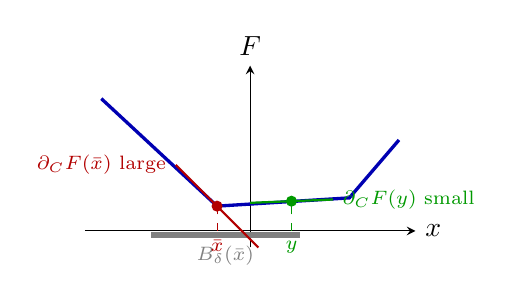
\begin{tikzpicture}[x=1.05cm,y=1.05cm,>=stealth]
    \draw[->] (-2,0) -- (2,0) node[right] {$x$};
    \draw[->] (0,-0.2) -- (0,2) node[above] {$F$};
    \draw[very thick,blue!70!black]
        (-1.8,1.6) -- (-0.4,0.3) -- (1.2,0.4) -- (1.8,1.1);
    \draw[gray,line width=2pt] (-1.2,-0.05) -- (0.6,-0.05);
    \node[gray] at (-0.3,-0.3) {\scriptsize $B_\delta(\bar x)$};
    \fill[red!70!black] (-0.4,0.3) circle (2pt);
    \node[below,red!70!black] at (-0.4,0) {\scriptsize $\bar x$};
    \draw[dashed,red!70!black] (-0.4,0) -- (-0.4,0.3);
    \draw[red!70!black,thick] (-0.9,0.8) -- (0.1,-0.2);
    \node[red!70!black,left] at (-0.9,0.8)
        {\scriptsize $\partial_C F(\bar x)$ large};
    \fill[green!60!black] (0.5,0.36) circle (2pt);
    \node[below,green!60!black] at (0.5,0) {\scriptsize $y$};
    \draw[dashed,green!60!black] (0.5,0) -- (0.5,0.36);
    \draw[green!60!black,thick] (0,0.34) -- (1,0.38);
    \node[green!60!black,right] at (1,0.38)
        {\scriptsize $\partial_C F(y)$ small};
\end{tikzpicture}

{\scriptsize Move to a nearby $y\in B_\delta(\bar x)$ where the
subgradient is small.}

\column{0.48\textwidth}
\centering
\textbf{VAC: value}

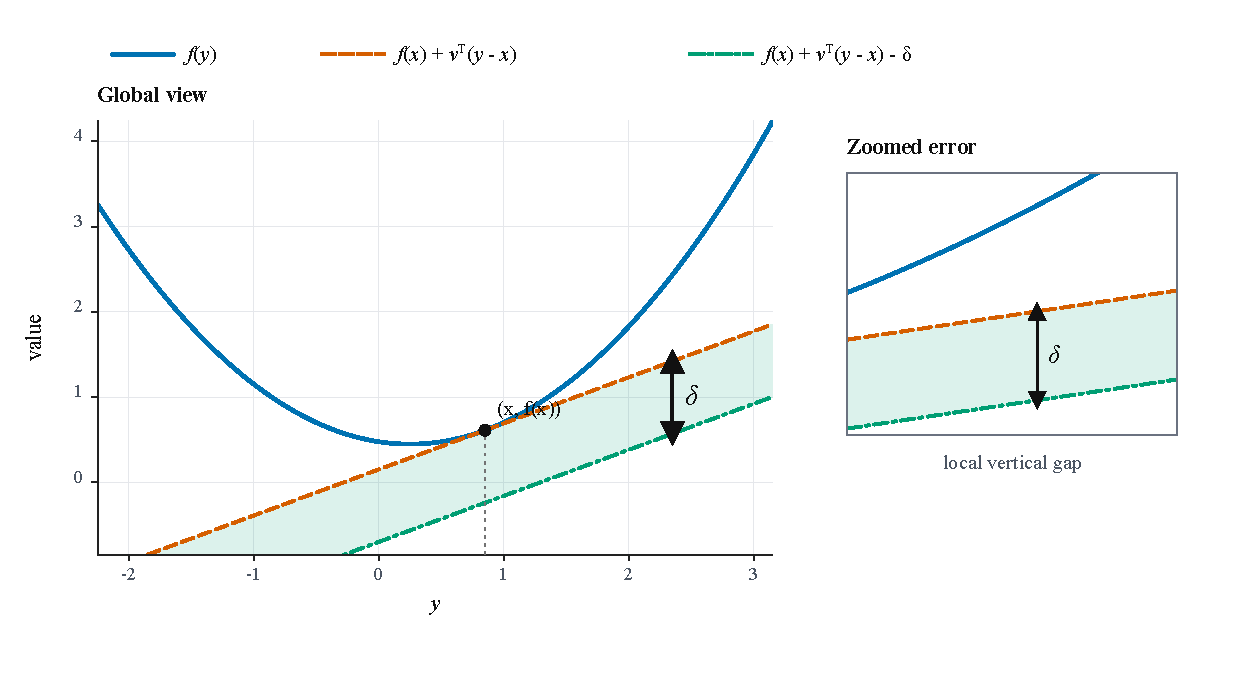
\includegraphics[
    width=0.94\linewidth,
    trim=0pt 21pt 226pt 43pt,
    clip
]
    {../figure/epsilon_subgradient.pdf}

{\scriptsize Stay at $\bar x$; shift the support\\[-2pt]
by a Fenchel gap.}
\end{columns}

\vspace{0.05cm}
\begin{center}
\scriptsize GAS and spatial NAS certify a neighborhood point; VAC keeps
the reported point fixed.
\end{center}
% \footnote{\footnotesize In this comparison, NAS means the spatial neighborhood notion.
% The Moreau/prox NAS used for the upper bound is distinct and implies
% $(\varepsilon/(2\rho),\varepsilon)$-GAS under weak convexity.}

\end{frame}

\begin{frame}{Nearly Approximate Stationarity (NAS)}
\footnotesize
\vspace{0.2cm}

Let $F$ be a $\rho$-weakly convex function with $\rho>0$ and define
\[
    F_{1/(2\rho)}(x):=\inf_y\{F(y)+\rho\|y-x\|^2\}.
\]

\medskip
\begin{block}{Definition (NAS)\footnotemark}
We call $x$
an $\varepsilon$-NAS point of $F$ if
\[
    \bigl\|\nabla F_{1/(2\rho)}(x)\bigr\|\le \varepsilon.
\]
Equivalently, if $\hat x=\operatorname{prox}_{F/(2\rho)}(x)$, then
\[
    \|x-\hat x\|\le\frac{\varepsilon}{2\rho},
\qquad
    \operatorname{dist} (0, \partial F(\hat x)) \leq \varepsilon.
\]
\end{block}

\footnotetext{\footnotesize Damek Davis and Dmitriy Drusvyatskiy, ``Stochastic Model-Based
Minimization of Weakly Convex Functions,'' \emph{SIAM J. Optim.},
vol.~29, no.~1, pp.~207--239, 2019.}

\medskip
\textbf{One DC Decomposition of $F$}
\[
    F=\phi-g,
    \qquad
    \phi(x)=F(x)+\rho\|x\|^2,
    \qquad
    g(x)=\rho\|x\|^2.
\]
Here $\phi$ is convex and $g$ is $2\rho$-smooth convex. Moreover,
\[
\begin{aligned}
x\text{ is }(0,\delta_\phi,0)\text{-VAC}
&\Longleftrightarrow
2\rho x\in\partial_{\delta_\phi}\phi(x).
\end{aligned}
\]
\end{frame}


\begin{frame}{Proposition 1: VAC--NAS Relations}
\footnotesize

\begin{block}{Proposition 1}
\medskip

\textbf{(i) NAS $\Longrightarrow$ VAC.}
Assume that $F$ is $L$-Lipschitz. For every $\varepsilon>0$,
\[
   x\text{ is an }\varepsilon\text{-NAS point}
   \quad\Longrightarrow\quad
   x\text{ is a }
   \biggl(0,\frac{L\varepsilon}{2\rho},0\biggr)\text{-VAC point}.
\]

\medskip

\textbf{(ii) VAC $\Longrightarrow$ NAS.}
Under the canonical decomposition
\[
   \phi=F+\rho\|\cdot\|^2,
   \qquad
   g=\rho\|\cdot\|^2,
\]
for every $\delta_\phi\ge0$,
\[
   x\text{ is a }(0,\delta_\phi,0)\text{-VAC point}
   \quad\Longrightarrow\quad
   x\text{ is a }\sqrt{8\rho\,\delta_\phi}\text{-NAS point}.
\]

In particular,
\[
   \delta_\phi\le\frac{\varepsilon^2}{8\rho}
   \quad\Longrightarrow\quad
   x\text{ is an }\varepsilon\text{-NAS point}.
\]
\end{block}
\end{frame}

\begin{frame}{Main Finding and Discussion}
\small

\textbf{Finding}
\begin{itemize}\setlength{\itemsep}{3pt}
    \item Weakly convex recovery: $g$ is smooth, while $\phi$ may be
    nonsmooth.
    \item Since $g$ is smooth,
    \[
        \partial_C F(x)=\partial\phi(x)- \nabla g(x).
    \]
        \item A $\phi$-subgradient at the output point \red{therefore must exist;} otherwise the
    target may be unreachable.
\end{itemize}

\medskip
\red{\textbf{Discussion}}
\begin{itemize}\setlength{\itemsep}{3pt}
    \item Given the nonuniqueness of DC decompositions, is this 
    weakly convex recovery sufficient to reflect the intrinsic DC structure,
    or does it only describe the selected decomposition and algorithm?

    \item  When specialized to weakly convex optimization, the DC decomposition violates the globally bounded component-subgradient assumption in our DC oracle definition; how should the function class and oracle model be reformulated?
\end{itemize}
\end{frame}

\begin{frame}{Nearly Approximate Criticality (NAC)}
\footnotesize
We say $x$ is an $(\varepsilon,\delta)$-NAS point of $f$ if
\[
    \operatorname{dist}\left(
        0,\,
        \bigcup_{y\in\mathbb{B}_{\delta}(x)}
        \partial f(y)
    \right)
    \le \varepsilon.
\]
% \begin{block}{Definition (Davis--Drusvyatskiy '19, Davis--Grimmer '19)}

% \end{block}

\begin{block}{Definition (Sun--Sun '23): $(\widehat\varepsilon,\delta)$-NAC\footnotemark}

Given $\widehat\varepsilon,\delta\ge0$, we call $x$ a
$(\widehat\varepsilon,\delta)$-NAC point for $F=\phi-g$ if


\[\operatorname{dist}\!\left(
0,\,
\partial\phi(x)
-
\bigcup_{y\in B_\delta(x)}\partial g(y)
\right)
\le\widehat{\varepsilon}.\]

\end{block}

\medskip
\begin{itemize}\setlength{\itemsep}{1pt}
    \item $\widehat\varepsilon$: dual-vector mismatch;
    \item $\delta$: spatial displacement between $x$ and $y$.
\end{itemize}

% \begin{alertblock}{Remark: the converse fails in general}
% For $g(t)=|t|$, $\phi(t)=(t-2\delta)^2$, and $x=2\delta>0$,
% $0\in\partial\phi(x)$ and $0\in\partial_{2\delta}g(x)$, so $x$ is
% $(0,0,2\delta)$-VAC. However, every $y\in[\delta,3\delta]$ satisfies
% $\partial g(y)=\{1\}$, so $x$ is not $(0,\delta)$-NAC.
% \end{alertblock}
\vfill
\footnotetext{\footnotesize Kaizhao Sun and Xu Andy Sun, ``Algorithms for Difference-of-Convex
Programs Based on Difference-of-Moreau-Envelopes Smoothing,''
\emph{INFORMS Journal on Optimization}, vol.~5, no.~4,
pp.~321--339, 2023.}
\end{frame}

\begin{frame}{NAC to VAC}
\begin{block}{Proposition: NAC to VAC}
Assume that $g$ is (locally) $G$-Lipschitz. Then
\[
    (\widehat\varepsilon,\delta)-\text{NAC}
    \ \blue{\Longrightarrow}\ 
    {(\widehat\varepsilon,0, 2G\delta)\text{-VAC}}.
\]
% \hfill{\scriptsize\cref{Sun and Sun, 2023}}
\end{block}


\begin{itemize}
    \item Note that the converse fails in general.
    \item \red{Under the  weakly convex split,}
\[
(\widehat\varepsilon,\delta)\text{-NAC}
    \quad\Longleftrightarrow\quad
    \operatorname{dist}\bigl(0,\partial_C F(x)\bigr)
    \le
    \widehat\varepsilon+2\rho\delta,
\]
\red{so it inherits the finite-time unattainability of approximate Clarke stationarity;} 
\end{itemize}

\end{frame}

\begin{frame}{Goldstein Approximate Stationarity (GAS)}
\small
\vspace{0.15cm}
\setlength{\abovedisplayskip}{2pt}
\setlength{\belowdisplayskip}{2pt}
\begin{block}{Definition (Goldstein '77; Burke--Lewis--Overton '05)}
For a locally Lipschitz $F$, we say that $z$ is a $(\varepsilon,\delta)$-GAS point if
\[
\operatorname{dist}\bigl(0,\operatorname{conv}\!\left(\bigcup_{y\in B_\delta(z)}
    \partial_C F(y)\right)\bigr)
    \le\varepsilon.
\]
\end{block}

% \medskip
% \textbf{Note.}
% Under the spatial NAS convention, $(\varepsilon,\delta)$-NAS is
% $(\varepsilon,\delta)$-GAS, but the converse generally fails. The
% Moreau/prox NAS used elsewhere instead implies
% $(\varepsilon/(2\rho),\varepsilon)$-GAS.

\medskip
\begin{block}{Proposition: GAS to VAC}
Assume that both convex components are (locally) $G$-Lipschitz. Then
\[
    (\varepsilon,\delta)\text{-GAS}
    \ \blue{\Longrightarrow}\ 
    {(\varepsilon,2G\delta,2G\delta)\text{-VAC}}.
\]
\end{block}

\vspace{-2pt}
{\footnotesize The implication uses
$\partial_C(\phi-g)(y)\subseteq\partial\phi(y)-\partial g(y)$ and
transports each component subgradient from $y\in B_\delta(z)$ to $z$.}


\end{frame}

% \begin{frame}{Q2. Nonsmooth $g$: Existing Treatment and the Gap}
% \footnotesize
% \begin{columns}[T,onlytextwidth]
% \column{0.48\textwidth}
% \begin{block}{Spatial DC certificates}
% For $v\in\partial g(y)$ with $\|x-y\|\le\delta$ and globally
% $G$-Lipschitz $g$,
% \[
%     \Phi_g(x,v)\le2G\delta,
%     \qquad v\in\partial_{2G\delta}g(x).
% \]
% Thus a nearby subgradient of nonsmooth $g$ is transported to a
% same-point \emph{value} tolerance.
% \end{block}

% \begin{block}{Moreau smoothing}
% For $v=\nabla g_\mu(x)$,
% \[
% \begin{gathered}
% v\in\partial g(\operatorname{prox}_{\mu g}(x)),\\[-2pt]
% \Phi_g(x,v)\le2G^2\mu.
% \end{gathered}
% \]
% Stationarity of a smooth surrogate therefore carries an implicit
% original-$g$ bias of order $\mu$.
% \end{block}

% \column{0.48\textwidth}
% \begin{block}{What VAC changes}
% VAC keeps the original nonsmooth $g$ and makes the transport or smoothing
% bias an explicit certificate slot $\delta_g$. In DCA, the transported
% vector $v^k\in\partial g(x^k)$ naturally yields the quantity
% \(\Phi_g(x^{k+1},v^k)\).
% \end{block}

% \begin{alertblock}{Literature gap to verify}
% The works reviewed here treat spatial DC certificates and smoothed-surrogate
% stationarity separately. We have not found an identical two-sided,
% same-point Fenchel-gap certificate that uses $\delta_g$ as their common
% comparison ledger; this should be checked before making a priority claim.
% \end{alertblock}
% \end{columns}
% \footnote{\footnotesize K.~Sun and X.~A.~Sun, ``Algorithms for Difference-of-Convex
% Programs Based on Difference-of-Moreau-Envelopes Smoothing,''
% INFORMS J. Optim., 2023.}
% \end{frame}
\begin{frame}{$\mathcal O(\varepsilon^{-4})$ First-Order Complexity Recovery}
\footnotesize

\begin{block}{Algorithm 1: Inexact DCA under $\mathcal O_{DC}$}
\begin{itemize}\setlength{\itemsep}{3pt}

    \item At the $k$-th iteration, consider the DCA subproblem
    \[
        \min_x\; F_{k}(x) = 
        \phi(x)-\langle\nabla g(x^k),x\rangle
        \equiv
        \min_x\;
        \left\{
        F(x)+\rho\|x-x^k\|^2
        \right\},
    \]
    which is $\rho$-strongly convex.

    \item \textbf{Inner solver:} Run $J$ subgradient descent steps on
    $B(x^k,G/\rho)$ to obtain $x^{k+1}$ satisfying
    \[
         F_{k}(x^{k+1})
        \le
        \inf_x\left\{
           F_{k}(x) 
        \right\}+a,
    \]
    where $a>0$ is the prescribed inner accuracy.

    \item \textbf{Output:} Define
    \[
        \bar\delta_k:=F_k(x^k)-F_k(x^{k+1})+a\ge0.
    \]
    Return $x^{k_\star}$, where
    $k_\star\sim\operatorname{Unif}\{0,\ldots,K-1\}$ with $K$ iteration.

\end{itemize}
\end{block}
    

    
\end{frame}

\begin{frame}{ $\mathcal O(\varepsilon^{-4})$ First-Order Complexity Recovery}
\scriptsize
\setlength{\abovedisplayskip}{2pt}
\setlength{\belowdisplayskip}{2pt}


\begin{block}{Theorem}
Let $F:\mathbb R^d\to\mathbb R$ be $\rho$-weakly convex with $\rho>0$
and $G$-Lipschitz, and let $\Delta_0:=F(x^0)-\inf F\in(0,\infty)$.
For any $\varepsilon>0$, set
\[
    a=\frac{\varepsilon^2}{16\rho},
    \qquad
    K=\left\lceil\frac{16\rho\Delta_0}{\varepsilon^2}\right\rceil,
    \qquad
    J=\mathcal O\!\left(\frac{G^2}{\varepsilon^2}\right).
\]
Then the output $x^{k_\star}$ is a
$(0,\bar\delta_{k_\star},0)$-AC point and, with expectation over $k_\star$,
\[
    \mathbb E\!\left[\bar\delta_{k_\star}\right]
    \le \frac{\varepsilon^2}{8\rho}
    \quad\Longrightarrow\quad
    \mathbb E\!\left[
        \bigl\|\nabla F_{1/(2\rho)}(x^{k_\star})\bigr\|^2
    \right]
    \le \varepsilon^2.
\]
The total first-order oracle complexity is
$\mathcal O(\rho\Delta_0G^2/\varepsilon^4)$.
\end{block}

\begin{alertblock}{Remark}
Through the AC-to-NAS bridge, Algorithm 1 recovers the standard
$\mathcal O(\varepsilon^{-4})$ first-order oracle complexity for weakly convex
near-stationarity in expectation.\footnotemark
\end{alertblock}

% \footnotemark
\vfill
\footnotetext{\tiny Jiajin Li and Siyu Pan, ``Optimal Deterministic Oracle Complexity
for Weakly Convex Optimization,'' arXiv:2608.03246, 2026.}

\end{frame}

\subsection{III. Q3}
\begin{frame}{Q3. DC Oracle Complexity: Five Core Objects}
\footnotesize
\begin{enumerate}\setlength{\itemsep}{4pt}
    \item \textbf{Problem instance.}
    \[
        I=(\phi,g),\qquad F_I=\phi-g.
    \]

    \item \textbf{Admissible class.}
    $I\in\mathcal D_{\mathrm{dc}}(\Delta,L,G)$, where $\Delta$ controls the
    initial gap, $L$ controls $F_I$, and $G$ controls component subgradients.

    \item \textbf{Information oracle.}
    At a query $x$, the algorithm observes
    \[
        \mathcal O_{\mathrm{dc}}(I,x)
        =\bigl(\phi(x),g(x),\partial\phi(x),\partial g(x)\bigr).
    \]

    \item \textbf{Algorithm and query sequence.}
    $\mathcal A\in\mathfrak A_{\mathrm{det}}(\mathcal O_{\mathrm{dc}})$ chooses
    $x_{\mathcal A[I]}^k$ using only the preceding oracle transcript.

    \item \textbf{Success criterion.}
    \[
    R_I(x):=\operatorname{dist}\!\left(0,\partial\phi(x)-\partial g(x)\right)
    =\inf_{\substack{u\in\partial\phi(x)\\v\in\partial g(x)}}\|u-v\|.
    \]
    A query is successful when $R_I(x)\le\varepsilon$.
\end{enumerate}
\end{frame}

\begin{frame}{Q3. Reading the Min--Max Hardness Statement}
\footnotesize
With the five objects fixed, the deterministic finite-budget statement is
\[
\underbrace{\inf_{\mathcal A\in\mathfrak A_{\mathrm{det}}(\mathcal O_{\mathrm{dc}})}}_
{\text{best algorithm}}
\underbrace{\sup_{I\in\mathcal D_{\mathrm{dc}}(\Delta,L,G)}}_
{\text{hardest admissible instance}}
\underbrace{\min_{0\le k<K}}_{\text{best queried point}}
R_I\!\left(x_{\mathcal A[I]}^k\right)
>\varepsilon.
\]

\begin{block}{Read the quantifiers from inside to outside}
\begin{enumerate}\setlength{\itemsep}{3pt}
    \item $\min_{k<K}$ gives the algorithm credit for its best point among
    the first $K$ queries.
    \item $\sup_I$ selects the hardest admissible DC pair after
    $\mathcal A$ has been fixed.
    \item $\inf_{\mathcal A}$ asks whether even the best deterministic
    algorithm can guarantee success.
\end{enumerate}
\end{block}

Equivalently, the target theorem has the quantifier form
\[
\forall\mathcal A\in\mathfrak A_{\mathrm{det}},\quad
\exists I\in\mathcal D_{\mathrm{dc}}(\Delta,L,G):\quad
R_I\!\left(x_{\mathcal A[I]}^k\right)>\varepsilon,
\quad k=0,\ldots,K-1.
\]

\begin{alertblock}{Current status}
The oracle model and minimax statement are fixed. A DC hard instance proving
this statement with budget-independent $(\Delta,L,G)$ is still missing.
\end{alertblock}
\footnote{\footnotesize Lai Tian and Anthony Man-Cho So,
``No Dimension-Free Deterministic Algorithm Computes Approximate
Stationarities of Lipschitzians,'' \emph{Mathematical Programming},
vol.~208, nos.~1--2, pp.~51--74, 2024, Theorem~1.}
\end{frame}

\section{Summary and Future Work}
\begin{frame}{Summary and Future Work}
\scriptsize
\begin{columns}[T,onlytextwidth]
\column{0.48\textwidth}
\textbf{What is established in this discussion}
\begin{itemize}\setlength{\itemsep}{1pt}
    \item VAC is a same-point, decomposition-dependent Fenchel-gap
    certificate; zero tolerances recover exact DC criticality.
    \item Under the canonical quadratic split, VAC and NAS are
    quantitatively linked, but not equivalent at the same tolerance.
    \item VAC differs from Clarke/Goldstein stationarity: it relaxes values
    at one point rather than sampling a neighborhood.
    \item Under an $F$-first-order oracle, inexact DCA gives an expected
    $\mathcal O(\varepsilon^{-4})$ NAS upper bound.
\end{itemize}

\column{0.48\textwidth}
\textbf{What remains open}
\begin{itemize}\setlength{\itemsep}{1pt}
    \item Q3: finite-time attainability of exact DC criticality under the
    component-wise DC oracle.
    \item Q3: a hard-instance construction with oracle
    indistinguishability and a DC-residual reduction.
    \item Q3: a common function class and oracle model for a meaningful
    DC upper/lower-complexity comparison.
\end{itemize}
\end{columns}

\vspace{0.15cm}
\begin{alertblock}{Takeaway}
VAC gives a finite-time same-point DC certificate; its NAS bridge is explicit,
while a matching DC-oracle lower bound remains open.
\end{alertblock}
\end{frame}

\ifshowappendix
\appendix
\begin{frame}{Appendix I: Proof of the NAC-to-VAC Reduction}
\footnotesize

\textbf{Proof.}
Let $x$ be an $(\widehat\varepsilon,\delta)$-NAC point. Then there
exist $y$, $u\in\partial\phi(x)$, and $v\in\partial g(y)$ such that
\[
    \|u-v\|\le\widehat\varepsilon,
    \qquad
    \|x-y\|\le\delta.
\]
Set
\[
    \bar\delta_g
    :=g(x)-g(y)-\langle v,x-y\rangle.
\]
By the subgradient inequality for $g$ at $y$, we have
$\bar\delta_g\ge0$ and, for every $z$,
\[
    g(z)
    \ge g(y)+\langle v,z-y\rangle
    =g(x)+\langle v,z-x\rangle-\bar\delta_g.
\]
Hence $v\in\partial_{\bar\delta_g}g(x)$. Moreover, since $g$ is
$G$-Lipschitz and $\|v\|\le G$,
\[
    \bar\delta_g
    \le |g(x)-g(y)|+\|v\|\,\|x-y\|
    \le 2G\|x-y\|
    \le 2G\delta.
\]
Therefore,
\[
    v\in\partial_{\bar\delta_g}g(x)
    \subseteq\partial_{2G\delta}g(x).
\]
Together with $u\in\partial\phi(x)$ and
$\|u-v\|\le\widehat\varepsilon$, this proves that $x$ is an
$(\widehat\varepsilon,0,2G\delta)$-VAC point.
\end{frame}

\begin{frame}{Appendix II: Proof of the NAS-to-VAC}
\footnotesize
\textbf{Setting.}
Use $\phi=F+\rho\|\cdot\|^2$ and $g=\rho\|\cdot\|^2$.
Let $\hat x=\operatorname{prox}_{F/(2\rho)}(x)$ and assume
$\|x-\hat x\|\le\varepsilon/(2\rho)$.

\medskip
\textbf{Choose the common witness.}
Set $u=v=\nabla g(x)=2\rho x$.
Then $\widehat\varepsilon=\|u-v\|=0$ and $\delta_g=0$.
Moreover, $u\in\partial_{\delta_\phi}\phi(x)$ is equivalent to
\[
    \phi(y)\ge\phi(x)+\langle2\rho x,y-x\rangle-\delta_\phi
    \qquad\forall y.
\]

\medskip
\textbf{Complete the square.}
After substituting $\phi=F+\rho\|\cdot\|^2$, the preceding inequality becomes
\[
    F(y)+\rho\|y-x\|^2\ge F(x)-\delta_\phi
    \qquad\forall y.
\]
Hence the smallest admissible tolerance is exactly
\[
    \delta_\phi^\star
    =F(x)-\inf_y\{F(y)+\rho\|y-x\|^2\}
    =F(x)-F_{1/(2\rho)}(x)\ge0.
\]
Finally,
\[
    \delta_\phi^\star
    =F(x)-F(\hat x)-\rho\|x-\hat x\|^2
    \le L\|x-\hat x\| 
    \le\frac{L\varepsilon}{2\rho}.
    \qquad\square
\]
\end{frame}

\begin{frame}{Appendix III: Proof of the VAC-to-NAS}
\footnotesize
Since $g$ is smooth, $(0,\delta_\phi,0)$-VAC forces
$u=v=\nabla g(x)=2\rho x$. Hence
\[
    2\rho x\in\partial_{\delta_\phi}\phi(x)
    \quad\Longleftrightarrow\quad
    F(y)+\rho\|y-x\|^2\ge F(x)-\delta_\phi
    \quad\forall y.
\]
Taking the infimum over $y$ gives
\[
    F(x)-F_{1/(2\rho)}(x)\le\delta_\phi.
\]
Conversely, this Moreau-gap bound implies the same
$\delta_\phi$-subgradient inequality, proving the equivalence.

\medskip
Let $x^+=\operatorname{prox}_{F/(2\rho)}(x)$. Since
$F(\cdot)+\rho\|\cdot-x\|^2$ is $\rho$-strongly convex,
\[
    \frac{\rho}{2}\|x-x^+\|^2
    \le F(x)-F_{1/(2\rho)}(x)
    \le\delta_\phi.
\]
Using $\nabla F_{1/(2\rho)}(x)=2\rho(x-x^+)$, we obtain
\[
    \bigl\|\nabla F_{1/(2\rho)}(x)\bigr\|
    \le\sqrt{8\rho\delta_\phi}.
    \qquad\square
\]
\end{frame}

\begin{frame}{Appendix IV: Expected Outer VAC Certificate}
\footnotesize
Let $x^{k+1}$ satisfy
\[
    Q_k(x^{k+1})\le\inf_y Q_k(y)+a,
    \qquad
    Q_k(y):=F(y)+\rho\|y-x^k\|^2-\rho\|x^k\|^2.
\]
Define
\[
    \bar\delta_k:=Q_k(x^k)-Q_k(x^{k+1})+a\ge0.
\]
Since $Q_k(x^{k+1})-a\le\inf Q_k$,
\[
\begin{aligned}
F(x^k)-F_{1/(2\rho)}(x^k)
&=Q_k(x^k)-\inf Q_k\\
&\le Q_k(x^k)-Q_k(x^{k+1})+a
 =\bar\delta_k.
\end{aligned}
\]
Therefore $x^k$ is a $(0,\bar\delta_k,0)$-VAC point.

\medskip
Also,
\[
\begin{aligned}
\bar\delta_k
&=F(x^k)-F(x^{k+1})-\rho\|x^{k+1}-x^k\|^2+a\\
&\le F(x^k)-F(x^{k+1})+a.
\end{aligned}
\]
For $k_\star\sim\operatorname{Unif}\{0,\ldots,K-1\}$,
\[
    \mathbb E[\bar\delta_{k_\star}]
    =\frac1K\sum_{k=0}^{K-1}\bar\delta_k
    \le\frac{\Delta_0}{K}+a.
\]
Taking $K\ge16\rho\Delta_0/\varepsilon^2$ and
$a=\varepsilon^2/(16\rho)$ gives
\[
\mathbb E[\bar\delta_{k_\star}]\le\frac{\varepsilon^2}{8\rho},
\qquad
\mathbb E\!\left[\|\nabla F_{1/(2\rho)}(x^{k_\star})\|^2\right]
\le\varepsilon^2.
\]
\end{frame}

\begin{frame}{Appendix V: Inner First-Order Complexity}
\footnotesize
Ignoring the constant $-\rho\|x^k\|^2$, the inner objective is
\[
    H_k(y):=F(y)+\rho\|y-x^k\|^2,
\]
which is $\rho$-strongly convex. If $y_k^\star=\arg\min_y H_k(y)$, then
$L$-Lipschitz continuity gives
\[
    \rho\|y_k^\star-x^k\|^2
    \le F(x^k)-F(y_k^\star)
    \le L\|y_k^\star-x^k\|,
\]
so $y_k^\star\in B(x^k,L/\rho)$.

\medskip
For $y\in B(x^k,L/\rho)$ and $s(y)\in\partial F(y)$,
\[
    q_k(y):=s(y)+2\rho(y-x^k)\in\partial H_k(y),
    \qquad
    \|q_k(y)\|\le3L.
\]
A projected weighted subgradient method with
\[
    y_{j+1}=\Pi_{B(x^k,L/\rho)}
    \bigl(y_j-\eta_jq_k(y_j)\bigr),
    \qquad \eta_j=\frac{2}{\rho(j+1)},
\]
and output
\[
    x^{k+1}=\frac{2}{J(J+1)}\sum_{j=1}^J j y_j
\]
therefore attains
\[
    H_k(x^{k+1})-H_k(y_k^*)
    \le\frac{18L^2}{\rho(J+1)}.
\]
Thus $J\ge288L^2/\varepsilon^2$ enforces
$a=\varepsilon^2/(16\rho)$.
The total count is $KJ+\mathcal O(K)$ first-order queries, since
the outer certificate needs $\mathcal O(K)$ function-value evaluations.
\medskip
Under the canonical split, each inner direction is obtained from one
first-order query to $F$:
\[
    \underbrace{s(y)+2\rho y}_{\in\partial\phi(y)}
    -\underbrace{2\rho x^k}_{=\nabla g(x^k)}
    =q_k(y).
\]
Hence the component-wise DC oracle and the displayed $F$-oracle have the
same information content for this canonical split.
\end{frame}

%   \begin{frame}{The Three Parameters: What Do They Measure?}
%   \small

%   \textbf{Recall the definition.} $(\delta_\phi,\delta_g,\widehat{\varepsilon})$-critical means: $\exists u,v$ with
%   \[
%       u\in\partial_{\delta_\phi}\phi(\bar x),
%       \qquad
%       v\in\partial_{\delta_g}g(\bar x),
%       \qquad
%       \|u-v\|\le\widehat{\varepsilon}.
%   \]

%   The three parameters separate independent sources of approximation error.

%   \medskip
%   \begin{itemize}\setlength{\itemsep}{2pt}
%       \item \textbf{$\delta_\phi$: subproblem solve accuracy.}

%        \blue{{\footnotesize How close did we get to the subproblem optimum?}}

%       \textit{In DCA:} Since $\min_x\{\phi(x)-\langle v^k,x\rangle\}=-\phi^*(v^k)$, we have
%   \[
%       \Phi_\phi(x^{k+1},v^k)
%       =\bigl\{\phi(x^{k+1})-\langle v^k,x^{k+1}\rangle\bigr\}
%       -\min_x\bigl\{\phi(x)-\langle v^k,x\rangle\bigr\},
%   \]
  

%       \item \textbf{$\delta_g$: nonsmooth transport cost.}

%       \blue{{\footnotesize How much Fenchel gap accumulates when using $v\in\partial g$ away from its anchor?}}

%       \textit{In DCA:} $v^k\in\partial g(x^k)$ moved to $x^{k+1}$ gives $\Phi_g(x^{k+1},v^k)$. 

%       \item \textbf{$\widehat{\varepsilon}$: dual-vector mismatch, not the stationarity residual.}

%       \blue{{\footnotesize How far apart are the two approximate subgradients?}}

%       \textit{In DCA:} at output $\bar x$, find $u\in\partial_{\delta_\phi}\phi(\bar x)$ and $v\in\partial_{\delta_g}g(\bar x)$, set
%   $\widehat{\varepsilon}=\|u-v\|$. Exact DCA may have $u=v=v^k$ and $\widehat{\varepsilon}=0$ while $\delta_g>0$; exact stationarity requires all three tolerances to vanish.
%   Proximal DCA: $u^k=v^k-\gamma\Delta x^{k}$, $\widehat{\varepsilon}=\gamma\|\Delta x^{k}\|$. 
%   \end{itemize}
%   \end{frame}

% \begin{frame}{Optimality Meaning}
%   \footnotesize

%   \textbf{Recall the motivating example:} $\Psi(x)=\bigl||x|-1\bigr|=\phi(x)-g(x)$ with
%   \[
%       \phi(x)=3+4(|x|-1)_+,
%       \qquad
%       g(x)=|x+1|+|x|+|x-1|.
%   \]

%   \begin{columns}[T,onlytextwidth]

%   \column{0.55\textwidth}

%   \textbf{The obstruction.}
%   Along the sequence $x_k=1-\frac{1}{k+2}\to1$:
%   \begin{itemize}\setlength{\itemsep}{1pt}
%       \item $0\in\partial\phi(1)-\partial g(1)$ (limit point is DC-critical);
%       \item yet $\operatorname{dist}\bigl(0,\partial\phi(x_k)-\partial g(x_k)\bigr)=1$ for every finite $k$ --- the traditional residual \red{jumps
%   at the kink}.
%   \end{itemize}

%   \column{0.4\textwidth}

%   \centering
%   \vspace{-0.8em}

%   \begin{tikzpicture}[x=0.75cm,y=1.25cm,>=stealth]

%       \draw[->] (-2.25,0) -- (2.25,0) node[right] {$x$};
%       \draw[->] (0,-0.15) -- (0,1.35) node[above] {$\Psi(x)$};

%       \draw[very thick,blue!70!black]
%           (-2,1) -- (-1,0) -- (0,1) -- (1,0) -- (2,1);

%       \fill[red!70!black] (-1,0) circle (2pt);
%       \fill[red!70!black] (1,0) circle (2pt);

%       \node[below] at (-1,0) {\scriptsize $-1$};
%       \node[below] at (1,0) {\scriptsize $1$};
%       \node[left] at (0,1) {\scriptsize $1$};

%   \end{tikzpicture}

%   \end{columns}

%   \medskip
%   \textbf{The new certificate isolates the failure.}
%   At any $x_k=1-\frac{1}{k+2}$:
%   \begin{itemize}\setlength{\itemsep}{1pt}
%       \item $\partial\phi(x_k)=\{0\}$ and $\partial g(x_k)=\{1\}$ (both are exact subgradients);
%       \item both Fenchel gaps are \emph{exactly zero}: $\Phi_\phi(x_k,0)=0$ and $\Phi_g(x_k,1)=0$;
%       \item the certificate reads $\blue{(0,0,1)}$ --- failure isolated in the \red{mismatch slot $\varepsilon=1$};
%       \item one DCA step from $x_k$ returns $\bar x=1$ with certificate $(0,0,0)$.
%   \end{itemize}

%   \medskip
%   \textbf{Why this matters.}
%   Fenchel gaps $\Phi_h(x,w)$ vary \emph{continuously} with $(x,w)$; the traditional residual $\operatorname{dist}(0,\partial\phi-\partial g)$ can
%   \emph{jump} at nonsmooth points.

%   $\Rightarrow$ The new certificate is \blue{finite-time diagnosable}: it tracks how close each component is to optimality, not just whether the
%   combined residual is small.
%   \end{frame}

% \begin{frame}{Spatial Relaxation vs. Value Relaxation}
% \footnotesize
% \vspace{0.4cm}
% \begin{itemize}
%     \item \textbf{$(\delta, \varepsilon)$-Goldstein stationary} \cref{Goldstein 1977; Zhang et al.\ 2020}:
%   $\operatorname{dist}(0,\partial_\delta^G F(z)) \leq \varepsilon$ where
%   $\partial_\delta^G F(z):=\operatorname{conv}\bigcup_{\|z'-z\|\le\delta}\partial_C F(z')$.
%   \item \textbf{Ours}: both certificates stay at the same point $\bar x$.
% \end{itemize}

  
%   \medskip
%     \begin{columns}[T,onlytextwidth]

%   \column{0.48\textwidth}
%   \centering
%   \textbf{Goldstein: spatial}

%   \begin{tikzpicture}[x=1.2cm,y=1.2cm,>=stealth]
%       % Axes
%       \draw[->] (-2,0) -- (2,0) node[right] {$x$};
%       \draw[->] (0,-0.2) -- (0,2) node[above] {$F$};

%       % Nonsmooth function (piecewise linear with kink)
%       \draw[very thick,blue!70!black]
%           (-1.8,1.6) -- (-0.4,0.3) -- (1.2,0.4) -- (1.8,1.1);

%       % Neighborhood interval
%       \draw[gray,line width=2pt] (-1.2,-0.05) -- (0.6,-0.05);
%       \node[gray] at (-0.3,-0.3) {\scriptsize $B_\delta(\bar x)$};

%       % Point x̄ (at kink, large subgradient)
%       \fill[red!70!black] (-0.4,0.3) circle (2pt);
%       \node[below,red!70!black] at (-0.4,0) {\scriptsize $\bar x$};
%       \draw[dashed,red!70!black] (-0.4,0) -- (-0.4,0.3);

%       % Subgradient at x̄ (steep)
%       \draw[red!70!black,thick] (-0.9,0.8) -- (0.1,-0.2);
%       \node[red!70!black,left] at (-0.9,0.8) {\scriptsize $\partial_C F(\bar x)$ large};

%       % Point y (away from kink, small subgradient)
%       \fill[green!60!black] (0.5,0.36) circle (2pt);
%       \node[below,green!60!black] at (0.5,0) {\scriptsize $y$};
%       \draw[dashed,green!60!black] (0.5,0) -- (0.5,0.36);

%       % Subgradient at y (nearly flat)
%       \draw[green!60!black,thick] (0,0.34) -- (1,0.38);
%       \node[green!60!black,right] at (1,0.38) {\scriptsize $\partial_C F(y)$ small};
%   \end{tikzpicture}

%   {\scriptsize Move to $y\in B_\delta(\bar x)$ where gradient is small}

%   \column{0.48\textwidth}
%   \centering
%   \textbf{Ours: value}

%   \begin{tikzpicture}[x=1.2cm,y=1.2cm,>=stealth]
%       % Axes
%       \draw[->] (-2,0) -- (2,0) node[right] {$x$};
%       \draw[->] (0,-0.2) -- (0,2) node[above] {$h$};

%       % Convex function (parabola)
%       \draw[very thick,blue!70!black,domain=-1.6:1.6,samples=50]
%           plot (\x,{0.5*\x*\x + 0.2});

%       % Point x̄
%       \fill[red!70!black] (0.8,0.52) circle (2pt);
%       \node[below,red!70!black] at (0.8,0) {\scriptsize $\bar x$};
%       \draw[dashed] (0.8,0) -- (0.8,0.52);

%       % Approximate subgradient (supporting line with gap)
%       \draw[green!60!black,thick,domain=-0.2:1.8]
%           plot (\x,{0.2*\x + 0.2});
%       \node[green!60!black,right] at (1.6,0.52) {\scriptsize  $v$};

%       % Fenchel gap (vertical distance)
%       \draw[red!70!black,thick,<->] (0.8,0.36) -- (0.8,0.52);
%       \node[red!70!black,right] at (0.85,0.44) {\scriptsize $\delta$};

%       % Label the gap
%       \draw[dashed,green!60!black] (0.8,0.36) -- (1.4,0.36);
%       \node[green!60!black,below] at (1.4,0.36) {\scriptsize $h(\bar x)+\langle v,\cdot-\bar x\rangle$};
%   \end{tikzpicture}

%   {\scriptsize Stay at $\bar x$, allow Fenchel gap $\le\delta$}

%   \end{columns}

%   \medskip
%  \textbf{Why value relaxation for DCA}
%   \begin{itemize}\setlength{\itemsep}{1pt}
%       \item Goldstein stationarity: requires additional mechanisms (smoothing or neighborhood sampling);
%       \item[ $\checkmark$] \textbf{$(\delta_\phi, \delta_g, \widehat{\varepsilon})$-criticality}:  uses quantities DCA already computes: $\Phi_\phi(x^{k+1},v^k)$ and $\Phi_g(x^{k+1},v^k)$.

%   \end{itemize}
%   \end{frame}
  
%   \begin{frame}{Exact Consistency and Unification}
%   % \footnotesize

%   \textbf{I. Exact consistency.}
%   $(\delta_\phi,\delta_g,\widehat{\varepsilon})\to0$ recovers exact DC criticality $0\in\partial\phi(\bar x)-\partial g(\bar x)$.

%   \medskip
%   \textbf{II. Unification of existing relaxations.}
%   \begin{itemize}\setlength{\itemsep}{2pt}
%       \item \textbf{Spatial notions} \cref{Moudafi 2021; Sun 2023; Yao 2022}:
%       offset $\|\bar x-\bar y\|$ becomes Fenchel slack
%       $2G\|\bar x-\bar y\|$ (Lipschitz) or $\tfrac{L}{2}\|\bar x-\bar y\|^2$ (smooth);

%       \item \textbf{Value-inexact DCA}: $\delta_\phi$ \emph{is} the subproblem gap --- no conversion needed;

%       \item \textbf{Goldstein stationarity} \cref{Zhang et al.\ 2020}: $(\delta,\varepsilon)$-Goldstein $\Rightarrow$
%   $(2G_\phi\delta,2G_g\delta,\widehat{\varepsilon})$-critical with
%   $\widehat{\varepsilon}:=\varepsilon$.

%   %     \textit{Key difference:} Goldstein searches spatially over $B_\delta(\bar x)$; ours relaxes duality gaps at $\bar x$ --- spatial vs value
%   % relaxation.
%   \end{itemize}

%   % \medskip
%   % \textbf{III. Why value relaxation for DCA?}
%   % Goldstein requires additional mechanisms (smoothing, neighborhood sampling). Our certificate is the \emph{natural output} of DCA's descent
%   % structure (next page).
%   \end{frame}

% \begin{frame}{One Identity for the DCA Family}
% \footnotesize
% DCA template:
% $v^k\in\partial g(x^k)$,\quad
% $x^{k+1}\approx\displaystyle\arg\min_x\bigl\{\phi(x)-\langle v^k,x\rangle\bigr\}$
% (+ prox).

% \medskip
% \textbf{One-step Fenchel-gap identity.}
% \[
%     F(x^k)-F(x^{k+1})
%     \;=\;
%     \underbrace{\Phi_\phi(x^k,v^k)}_{\text{current }\phi\text{-gap}}
%     \;+\;
%     \underbrace{\Phi_g(x^{k+1},v^k)}_{g\text{-transport}}
%     \;-\;
%     \underbrace{\Phi_\phi(x^{k+1},v^k)}_{\text{injected inexactness}} .
% \]
% An equality, not an inequality: it uses
% $g(x^k)+g^*(v^k)=\langle v^k,x^k\rangle$ only.

% \medskip
% \textbf{Every variant enters the same ledger.}
% \begin{itemize}\setlength{\itemsep}{1pt}
%     \item exact DCA: $\Phi_\phi(x^{k+1},v^k)=0$
%     $\Rightarrow$ certificate $\bigl(0,\,\Phi_g(x^{k+1},v^k),\,0\bigr)$;
%     \item inexact solve: $\Phi_\phi(x^{k+1},v^k)\le\sigma$
%     $\Rightarrow$ $\delta_\phi=\sigma$;
%     \item proximal DCA: the prox term creates the mismatch slot $\varepsilon$;
%     \item PS-DCA / stochastic: estimation error $\bar V$ enters the Fenchel
%     slots as $O(\bar V)$ and the mismatch slot as $O(\sqrt{\bar V})$.
% \end{itemize}
% \end{frame}



% \begin{frame}{Complexity Recovered and Tightness}
% \scriptsize
% $\Delta_0:=F(x^0)-F^\star$.
% \begin{center}
% \begin{tabular}{@{}lll@{}}
% \toprule
% \textbf{method} & \textbf{certificate after} $K$ \textbf{iterations} & \textbf{complexity}\\
% \midrule
% exact DCA & $\bigl(0,\frac{\Delta_0}{K},0\bigr)$ & $K=O\bigl(\frac{\Delta_0}{\delta_g}\bigr)$\\[3pt]
% inexact DCA & $\bigl(\sigma,\frac{\Delta_0}{K}+\sigma,0\bigr)$ & outer $O\bigl(\frac{\Delta_0}{\delta_g-\sigma}\bigr)$\\[3pt]
% % PS-DCA & $\bigl(0,\frac{\Delta_0}{K},O(K^{-1/2})\bigr)$ & $O\bigl(\max\bigl\{\frac{\Delta_0}{\delta_g},\frac{L_f\Delta_0}{\varepsilon^2}\bigr\}\bigr)$\\[3pt]
% proximal DCA & $\bigl(0,\frac{\Delta_0}{K},\sqrt{\frac{\Delta_0}{\gamma K}}\bigr)$ & $O\bigl(\max\bigl\{\frac{\Delta_0}{\delta_g},\frac{\Delta_0}{\gamma\varepsilon^2}\bigr\}\bigr)$\\[3pt]
% stochastic minibatch & $(O(\varepsilon^2),O(\varepsilon^2),\varepsilon)$ & $O\bigl(\sigma^2L_f\Delta_0\,\varepsilon^{-4}\bigr)$ SFO\\[3pt]
% % MVR / recursive momentum & $(O(\varepsilon^2),O(\varepsilon^2),\varepsilon)$ & $O\bigl(\sigma L_f\Delta_0\,\varepsilon^{-3}\bigr)$ SFO\\
% \bottomrule
% \end{tabular}
% \end{center}

% \medskip
% \textbf{Takeaways.}
% \begin{itemize}\setlength{\itemsep}{1pt}
%     \item all rows follow from one identity: the $g$-gap is part of each
%     step's descent, hence $\delta_g\le\Delta_0/K$ after $K$ steps;
%     \item exact DCA has zero mismatch when one vector certifies both
%     relaxed component conditions ($u=v=v^k$); this does not imply
%     $R_{\rm DC}=0$ while $\delta_g>0$. Prox shifts the mismatch by
%     $\gamma\|\Delta x\|$; stochastic gradients add $\sqrt{\bar V}$;
%     \item $L_g$-smooth $g$: choosing
%     $\delta_g=O(\varepsilon_{\rm stat}^2/L_g)$ converts the relaxed
%     certificate to classical $\varepsilon_{\rm stat}$-stationarity, so
%     $O(\varepsilon_{\rm stat}^{-2})$ cannot be improved;
%     \item nonsmooth $g$: whether $O(\varepsilon^{-2})$ is optimal? \red{open.}
% \end{itemize}

% \medskip
% \blue{\textbf{Contribution (to our knowledge).}}\; the first
% \emph{non-asymptotic} complexity analysis of DCA-type methods for
% nonsmooth $g$ that (i) does not smooth $g$ and (ii) returns a optimality guarantee measure.

% \end{frame}



% \begin{frame}{Discussion: Open Questions}
% % \footnotesize
% \begin{itemize}\setlength{\itemsep}{3pt}
%     \item \textbf{meaning of $\widehat{\varepsilon}$:} it is $0$, $\gamma\|\Delta x\|$,
%     or $\sqrt{\bar V}$ depending on the method: does this distance have
%     a geometric meaning in the dual space?
%     \item \textbf{lower bound, nonsmooth $g$:} are $\Omega(\widehat{\varepsilon}^{-2})$
%     component-wise queries necessary for a
%     $(\delta_\phi,\delta_g,\widehat{\varepsilon})$-critical point? can the
%     hard-instance ideas of the barrier theorem be reused?
%     \item \textbf{decomposition dependence:} the certificate depends on the
%     split $(\phi,g)$, not only on $F$ --- acceptable, since DCA itself uses
%     the split? is there a best split for a given budget?
%     % \item \textbf{stochastic case:} estimation error $\bar V$ enters the
%     % value gaps linearly but the mismatch as $\sqrt{\bar V}$ --- is this why
%     % variance reduction improves $O(\varepsilon^{-4})$ to $O(\varepsilon^{-3})$?
%     % \item \textbf{$\delta_\phi=0$ at every step} for single-loop exact
%     % solves --- should the inexact (double-loop) analysis stay in the talk?
% \end{itemize}
% \end{frame}



% \section{Summary}

% \begin{frame}{Summary}
% % \footnotesize
% \begin{enumerate}\setlength{\itemsep}{4pt}

% \item[\textbf{C1.}] \textbf{Unattainability of same-point $\varepsilon$-criticality.}
%       % We diagnose that classical same-point $\varepsilon$-criticality is
%       % subject to a \textbf{finite-query barrier} under the component-wise
%       % DC oracle, and redesign the stationarity target accordingly ---
%       % rather than proposing another DCA variant for an unverifiable target.

% \item[\textbf{C2.}] \textbf{A same-point, three-parameter criticality definition with optimality guarantee.}
%       % The $(\delta_\varphi,\delta_g,\varepsilon)$-critical point separates
%       % subproblem solve error, nonsmooth transport cost, and dual mismatch ---
%       % three sources conflated in prior residuals --- while remaining
%       % asymptotically exact and unifying $\varepsilon$-criticality, Goldstein
%       % stationarity, and the Frank--Wolfe DC gap.

% \item[\textbf{C3.}] \textbf{Unified Analysis framework for the whole DCA family.}
%       % A one-step Fenchel-gap accounting identity pins down where each
%       % variant's error lives: $\delta_g$ alone for exact DCA, $\delta_\varphi$
%       % for inexact solves, $\varepsilon$ for proximal steps, both scales for
%       % stochastic estimation.

% \item[\textbf{C4.}] \textbf{Complexity recovered without smoothing $g$.}
%       % Under the natural scaling $\delta_\varphi,\delta_g=O(\varepsilon^2)$:
%       % deterministic proximal DCA attains $O(\varepsilon^{-2})$; stochastic
%       % minibatch attains $O(\varepsilon^{-4})$; recursive-momentum (MVR)
%       % matches the $O(\varepsilon^{-3})$ benchmark exponent.

% \end{enumerate}

% % \medskip
% % \blue{\textbf{To our knowledge:}} the first \emph{non-asymptotic} DCA
% % complexity analysis for nonsmooth $g$: no smoothing of $g$, and the
% % certificate recovers exact DC criticality as tolerances vanish.
% \end{frame}

% \begin{frame}{Open questions}
% \footnotesize
% \begin{itemize}\setlength{\itemsep}{3pt}
% \item DC criticality reveals the basic same-point obstruction.
% \item Multiblock GS adds outer-point, multiplier, and Jacobian gaps.
% \item Goldstein relaxation absorbs the outer-point gap.
% \item Convex-combination bridging avoids the assembly condition.
% \item Shared-multiplier design removes $\eta_k$; descent controls transport errors.
% \end{itemize}

% \vspace{0.08cm}
% \textbf{Open questions:}
% \begin{enumerate}\setlength{\itemsep}{2pt}
% \item Which shared-multiplier route admits a finite-time proof?
% \item What blockwise Jacobian assumptions suffice for GS descent?
% \item When is chain-rule Goldstein stationarity equivalent to standard Goldstein stationarity?
% \end{enumerate}
% \end{frame}



\fi
\end{document}
